\documentclass{article}
\usepackage{hyperref}
\setlength{\paperwidth}{21cm}   % A4
\setlength{\paperheight}{29.7cm}% A4
\setlength\topmargin{-0.5cm}    
\setlength\oddsidemargin{0cm}   
\setlength\textheight{24.7cm} 
\setlength\textwidth{16.0cm}
\setlength\columnsep{0.6cm}  
\newlength\titlebox 
\setlength\titlebox{5cm}
\setlength\headheight{5pt}   
\setlength\headsep{0pt}


\usepackage[english]{babel}
\usepackage[utf8]{inputenc}
% Importing Graphics
\usepackage{graphicx}

\usepackage{listings}

% Colors for code
\usepackage{xcolor}
\definecolor{codegreen}{rgb}{0,0.6,0}
\definecolor{codegray}{rgb}{0.5,0.5,0.5}
\definecolor{codepurple}{rgb}{0.58,0,0.82}
\definecolor{backcolour}{rgb}{0.95,0.95,0.92}

\lstdefinestyle{mystyle}{
	commentstyle=\color{codegreen},
	keywordstyle=\color{magenta},
	numberstyle=\tiny\color{codegray},
	stringstyle=\color{codepurple},
	basicstyle=\ttfamily\footnotesize,
	breakatwhitespace=false,         
	breaklines=true,                 
	captionpos=b,                    
	keepspaces=true,                 
	numbers=left,                    
	numbersep=5pt,                  
	showspaces=false,                
	showstringspaces=false,
	showtabs=false,                  
	tabsize=2
}

\lstset{style=mystyle}

\title{CSE 4020 Machine Learning \\ Lab Assessment - 5  }
\author{Sujay Kumar M 20BDS0294\\ \small Computer Science Engineering with Specialization with DataScience\\ \tt sujaykumarreddy.m2020@vitstudent.ac.in
	\\ \url{https://github.com/sujaykumarmag/CSE4020}}



\begin{document}
\maketitle
\section{Dataset}
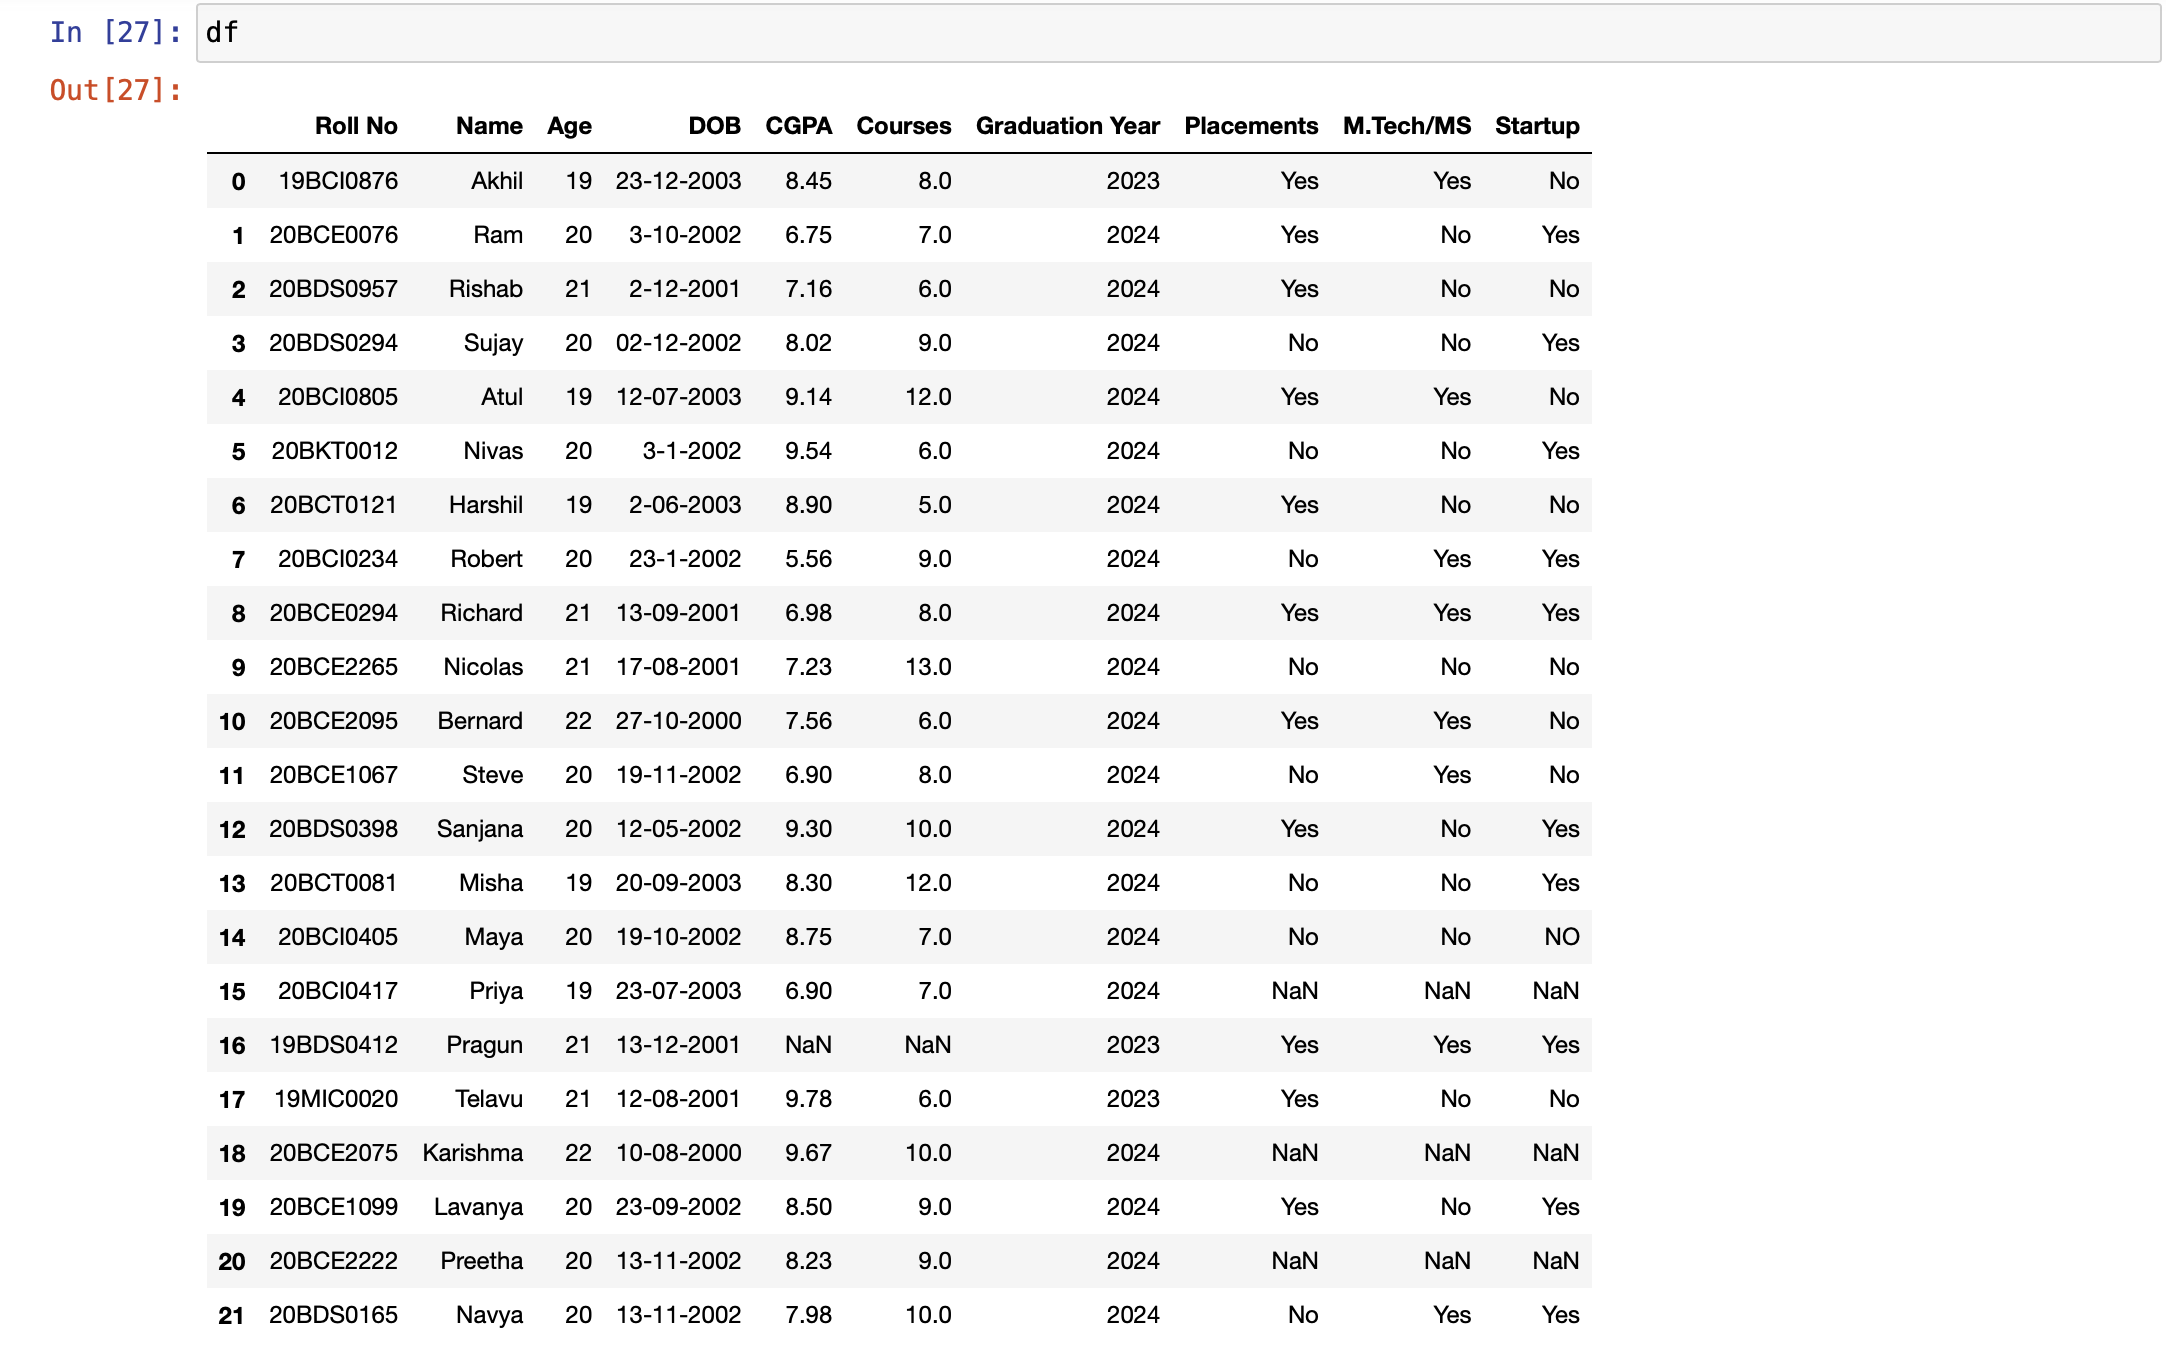
\includegraphics[scale=0.45]{images/1.png}
\break
\section{PreProcessing}
\begin{lstlisting}[language=Python]
	
	df = df.dropna(axis=0)
	data = df.drop(["Roll No","Name","DOB","M.Tech/MS","Startup"],axis=1)
	data["Placements"] = data["Placements"].apply(lambda row: 1 if row=="Yes" else 0)
\end{lstlisting}	
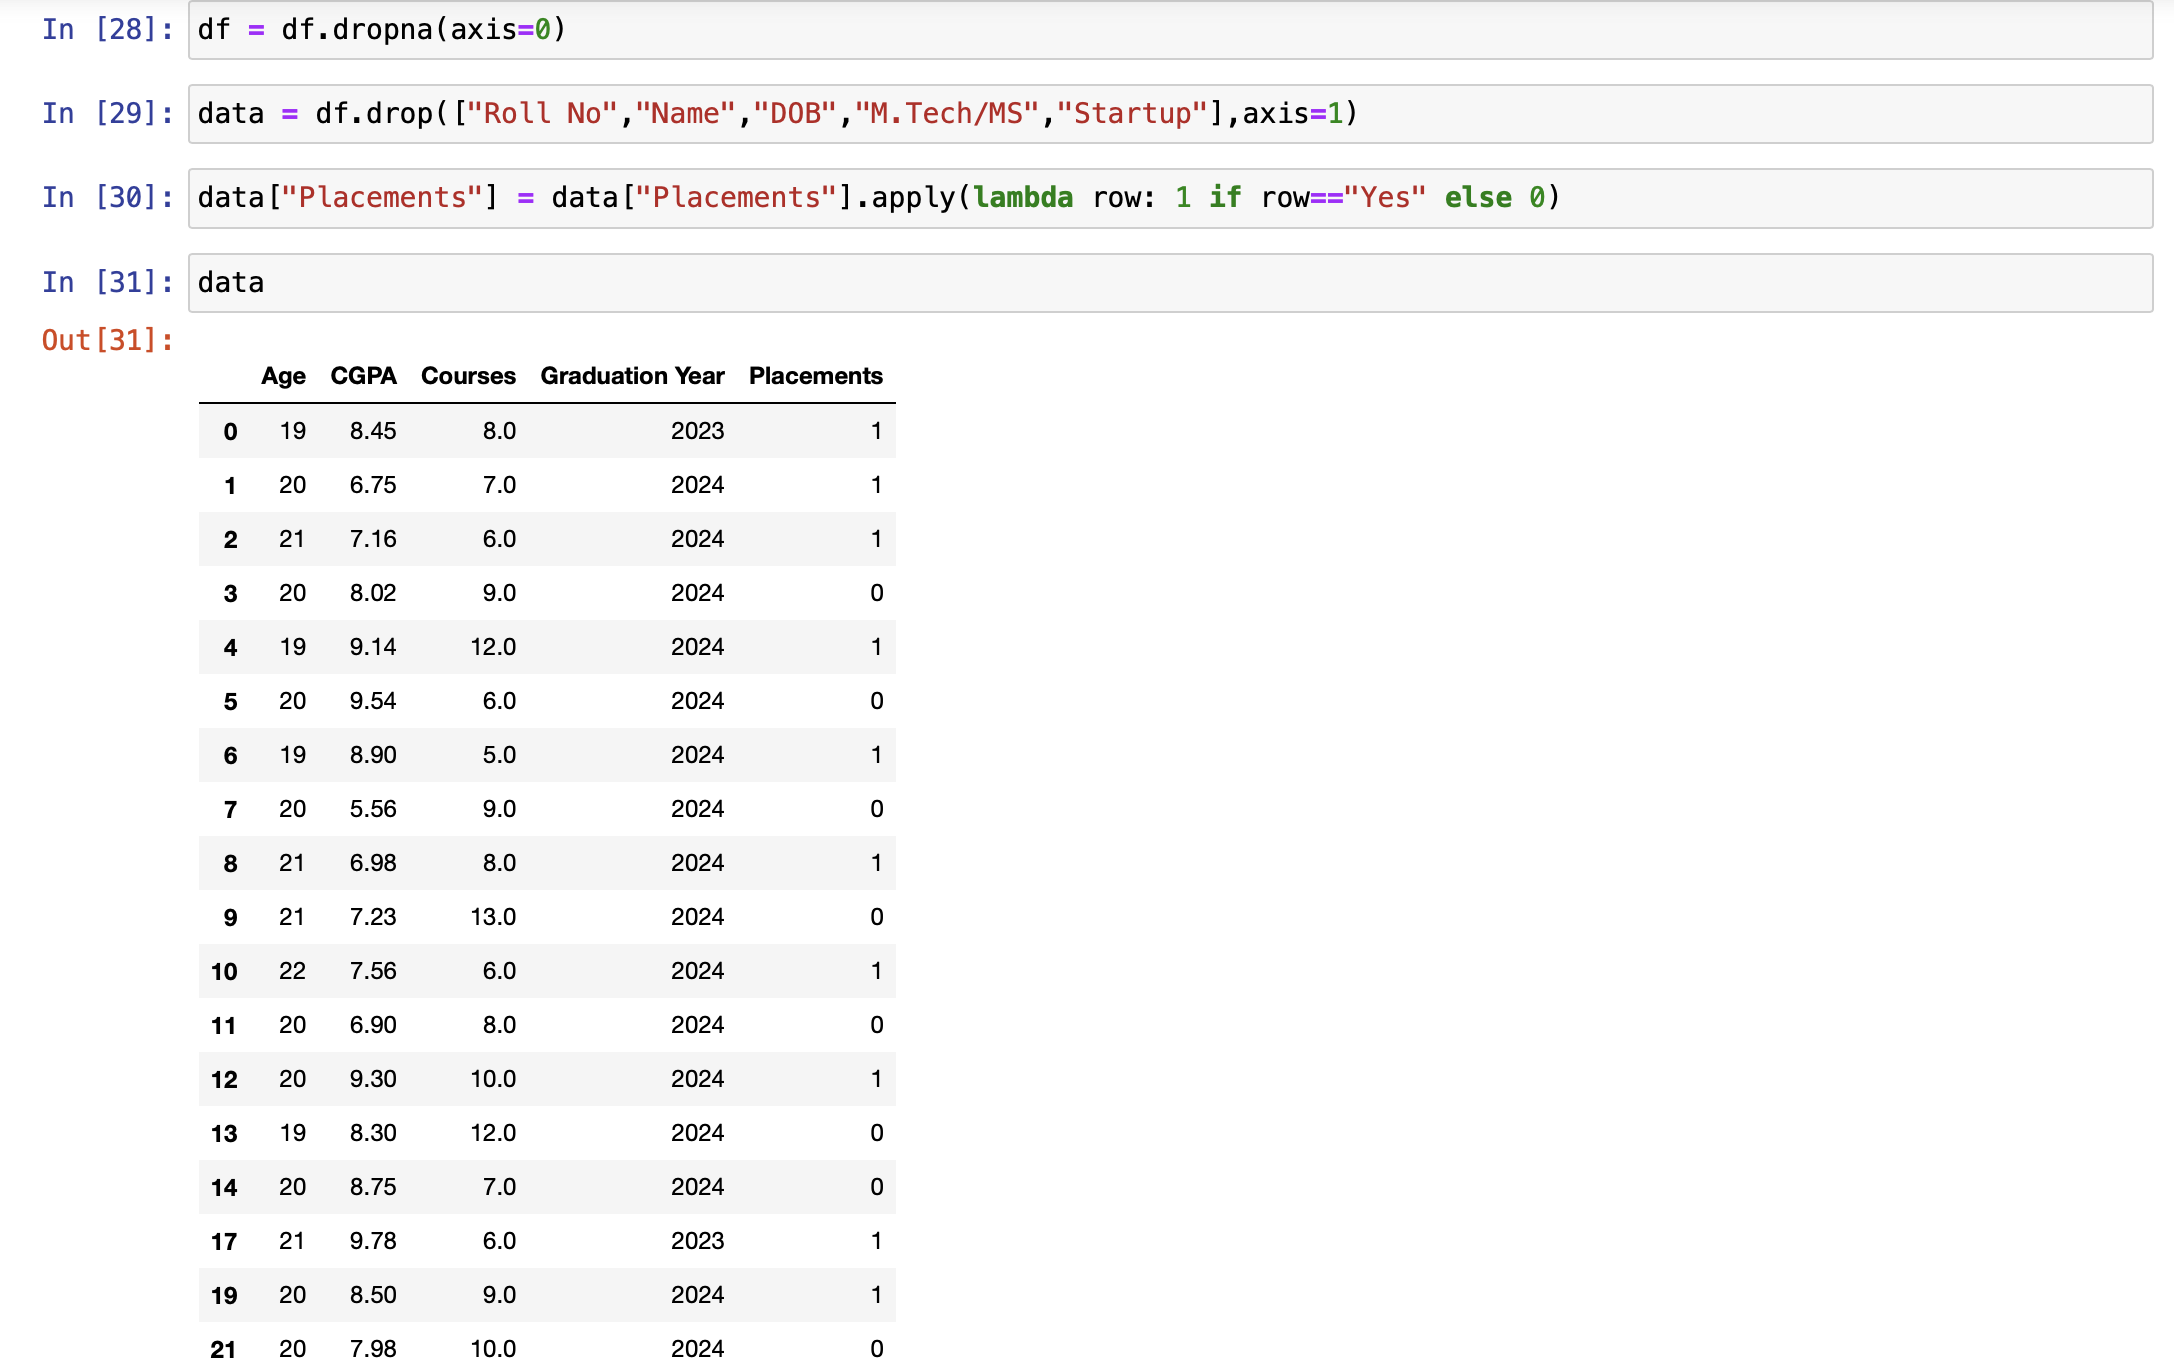
\includegraphics[scale=0.45]{images/2.png}
\section{Applying Standard Scalar for PCA}
\begin{lstlisting}[language=Python]
	from sklearn.preprocessing import StandardScaler
	features = ['Age', 'CGPA', 'Courses','Graduation Year']
	x = data.loc[:, features].values
	y = data.loc[:,['Placements']].values
	x = StandardScaler().fit_transform(x)
	x
\end{lstlisting}
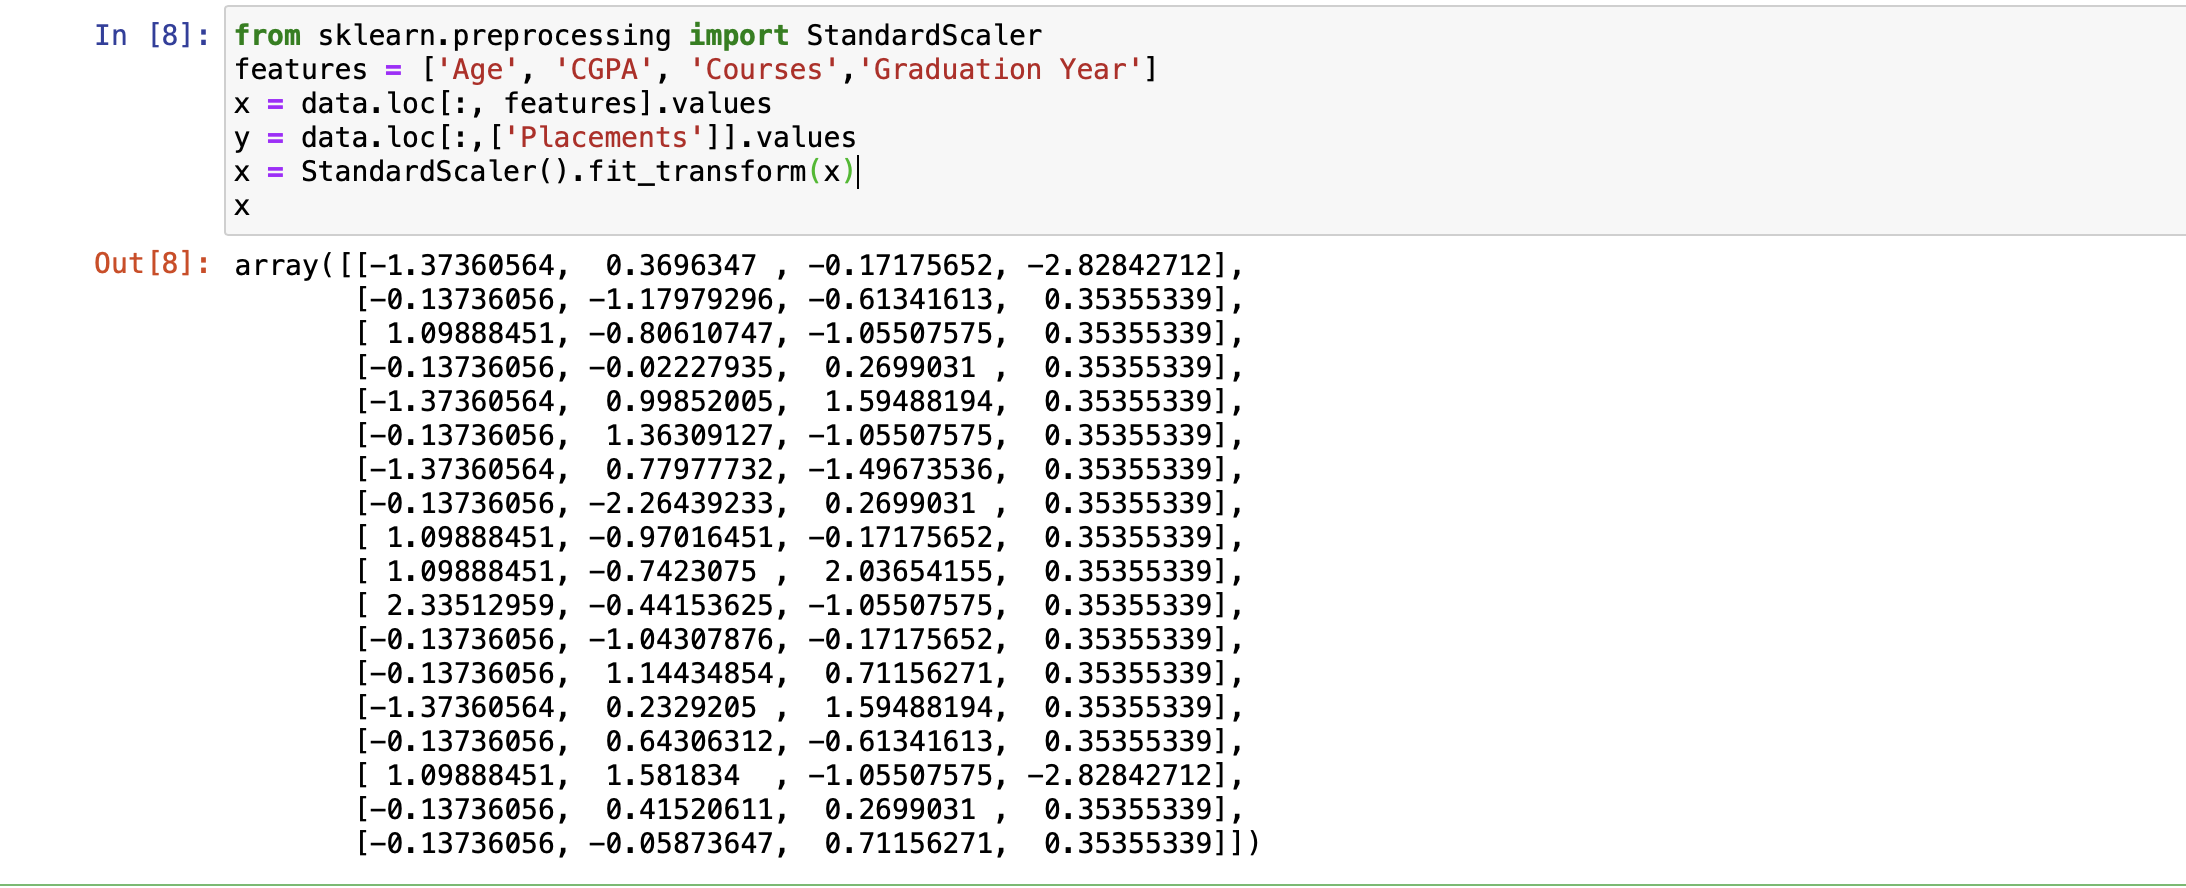
\includegraphics[scale=0.45]{images/3.png}
\section{Applying PCA}
\begin{lstlisting}[language=Python]
	from sklearn.decomposition import PCA
	pca = PCA(n_components=2)
	principalComponents = pca.fit_transform(x)
	principalDf = pd.DataFrame(data = principalComponents, columns = ['principal component 1', 'principal component 2'])
	finalDf = pd.concat([principalDf, data[['Placements']]], axis = 1)
	finalDf = finalDf.dropna(axis=0)
\end{lstlisting}
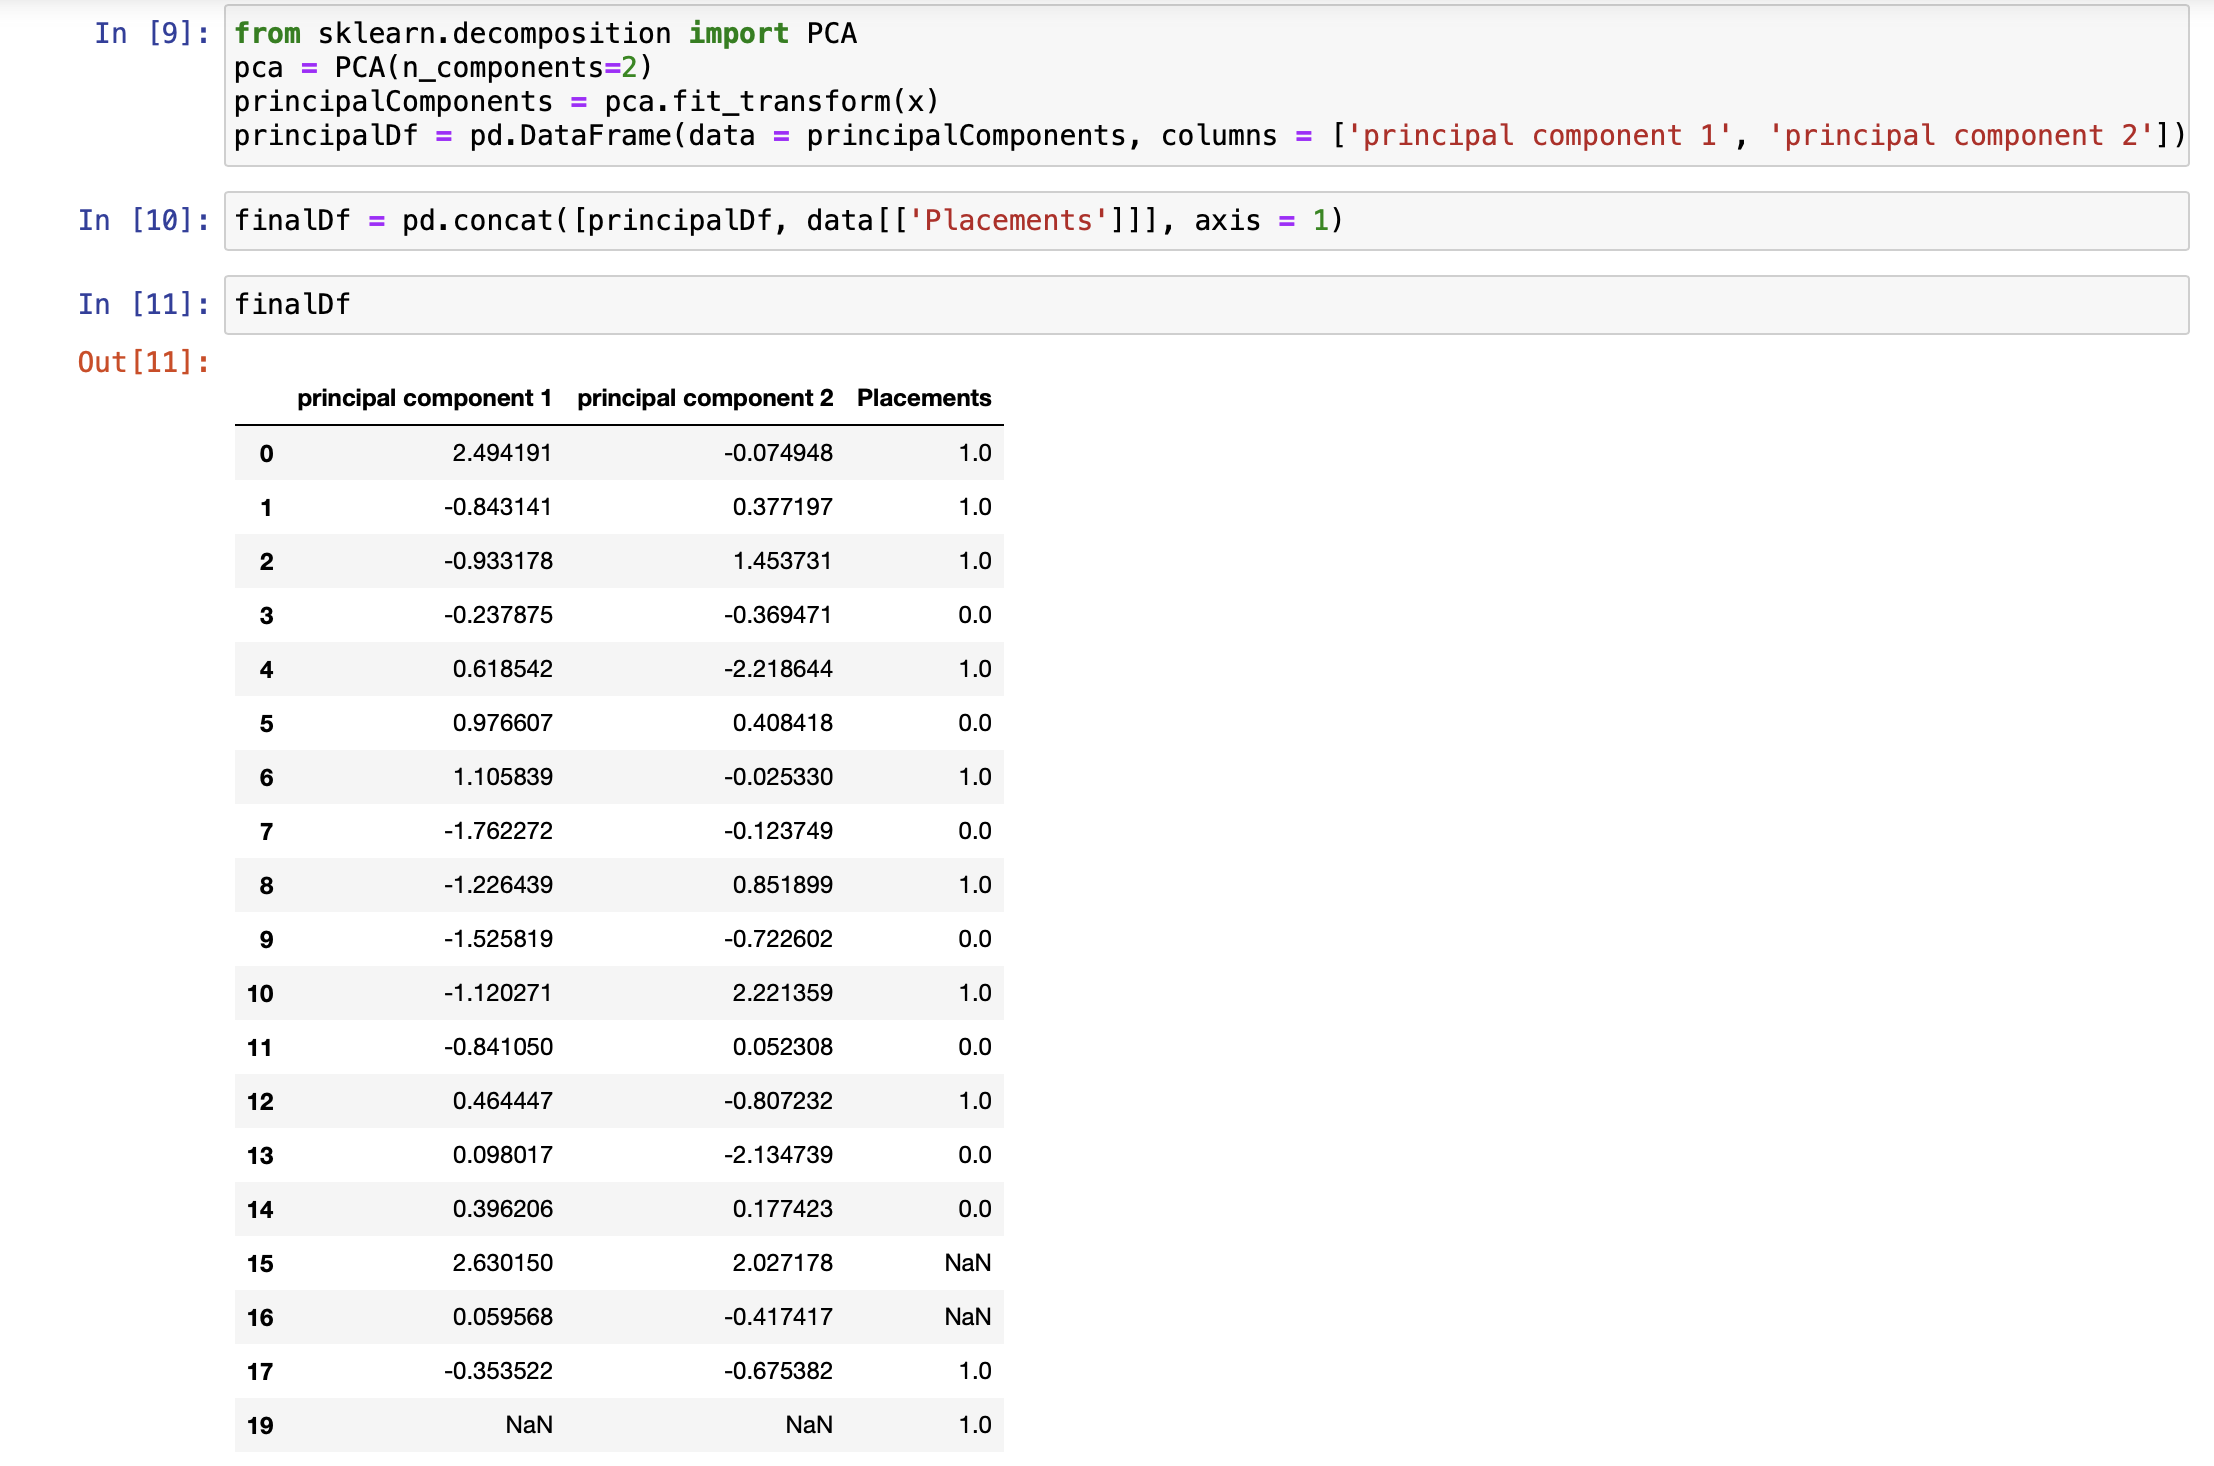
\includegraphics[scale=0.45]{images/4.png}
\section{Applying Logistic Regression Without PCA }
\begin{lstlisting}[language=Python]
	from sklearn.linear_model import LogisticRegression
	from sklearn.model_selection import train_test_split
	from sklearn.metrics import classification_report,accuracy_score
	
	
	X = data[["Age","CGPA","Courses","Graduation Year"]]
	y = data[["Placements"]]
	X_train, X_test,y_train,y_test = train_test_split(X,y,random_state=1)
	
	model1 = LogisticRegression()
	model1.fit(X_train,y_train)
	y_pred = model1.predict(X_test)
	print(accuracy_score(y_pred,y_test))
	print(classification_report(y_pred,y_test))
	
	
\end{lstlisting}
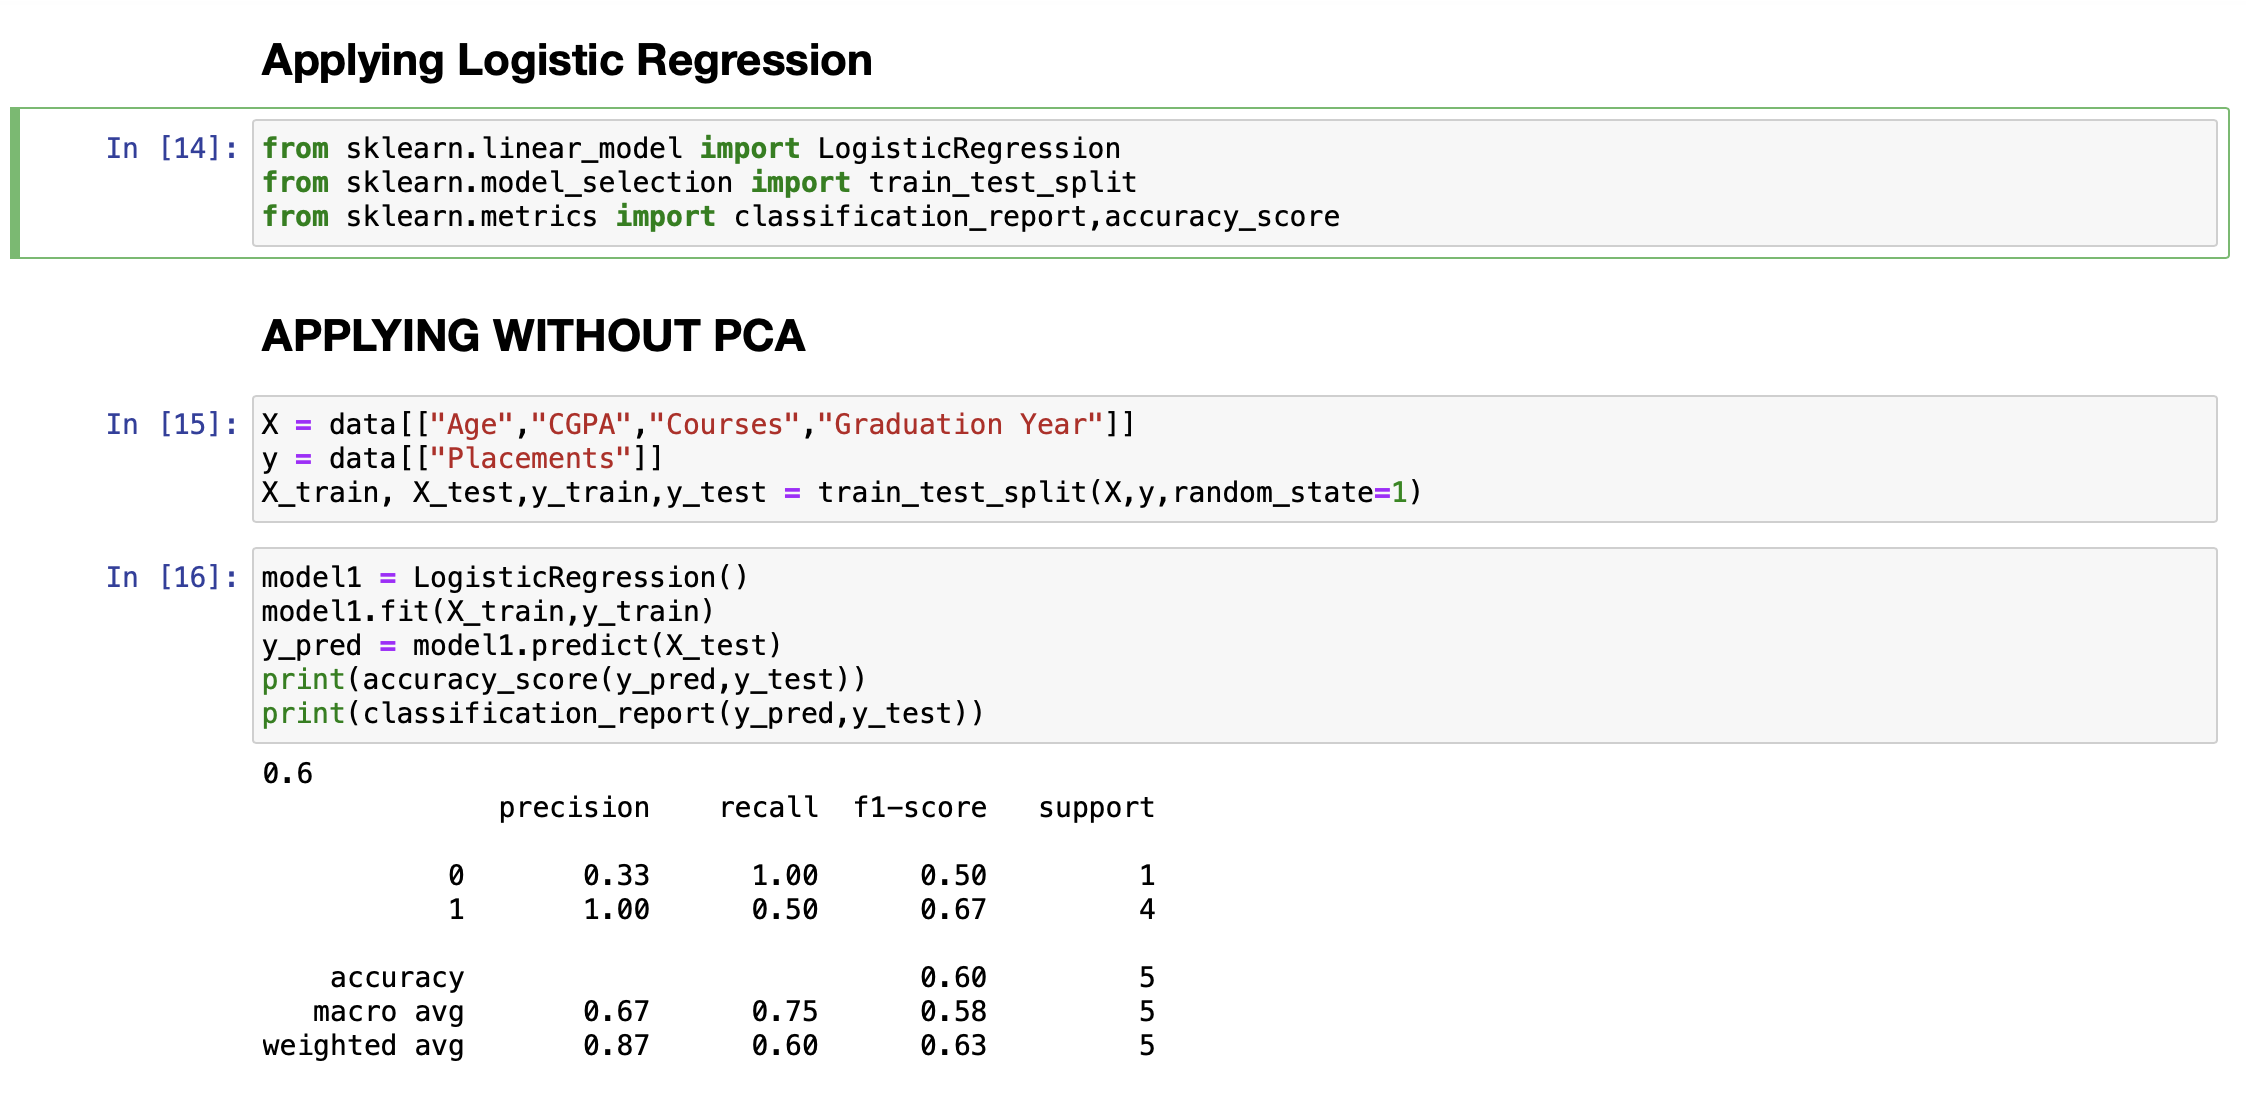
\includegraphics[scale=0.45]{images/6.png}
\section{Applying Logistic Regression with PCA}
\begin{lstlisting}[language=Python]
	X1 = finalDf[["principal component 1","principal component 2"]]
	y1 = finalDf[["Placements"]]
	X_train, X_test,y_train,y_test = train_test_split(X1,y1,random_state=23)
	
	model1 = LogisticRegression()
	model1.fit(X_train,y_train)
	y_pred = model1.predict(X_test)
	print(accuracy_score(y_pred,y_test))
	print(classification_report(y_pred,y_test))
	
\end{lstlisting}
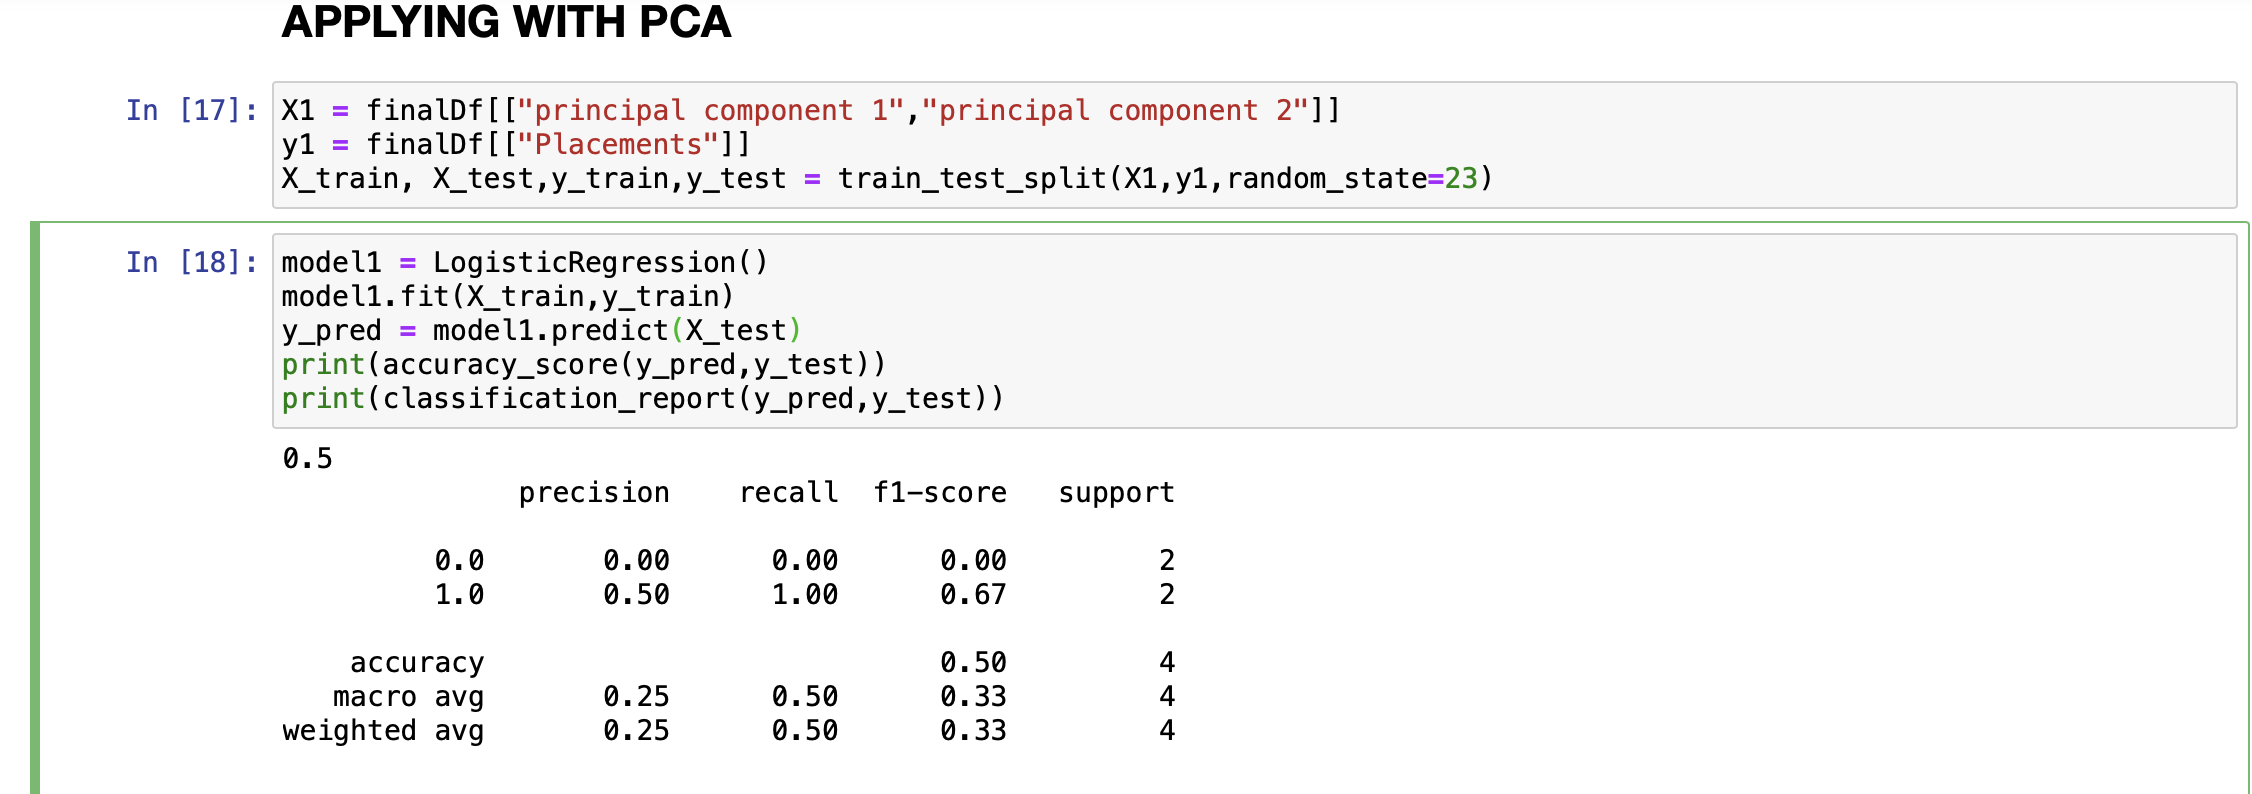
\includegraphics[scale=0.4]{images/7.png}
\section{Taking Care of Imbalanced data}
\begin{lstlisting}[language = Python]
	df["Placements"].value_counts()
\end{lstlisting}
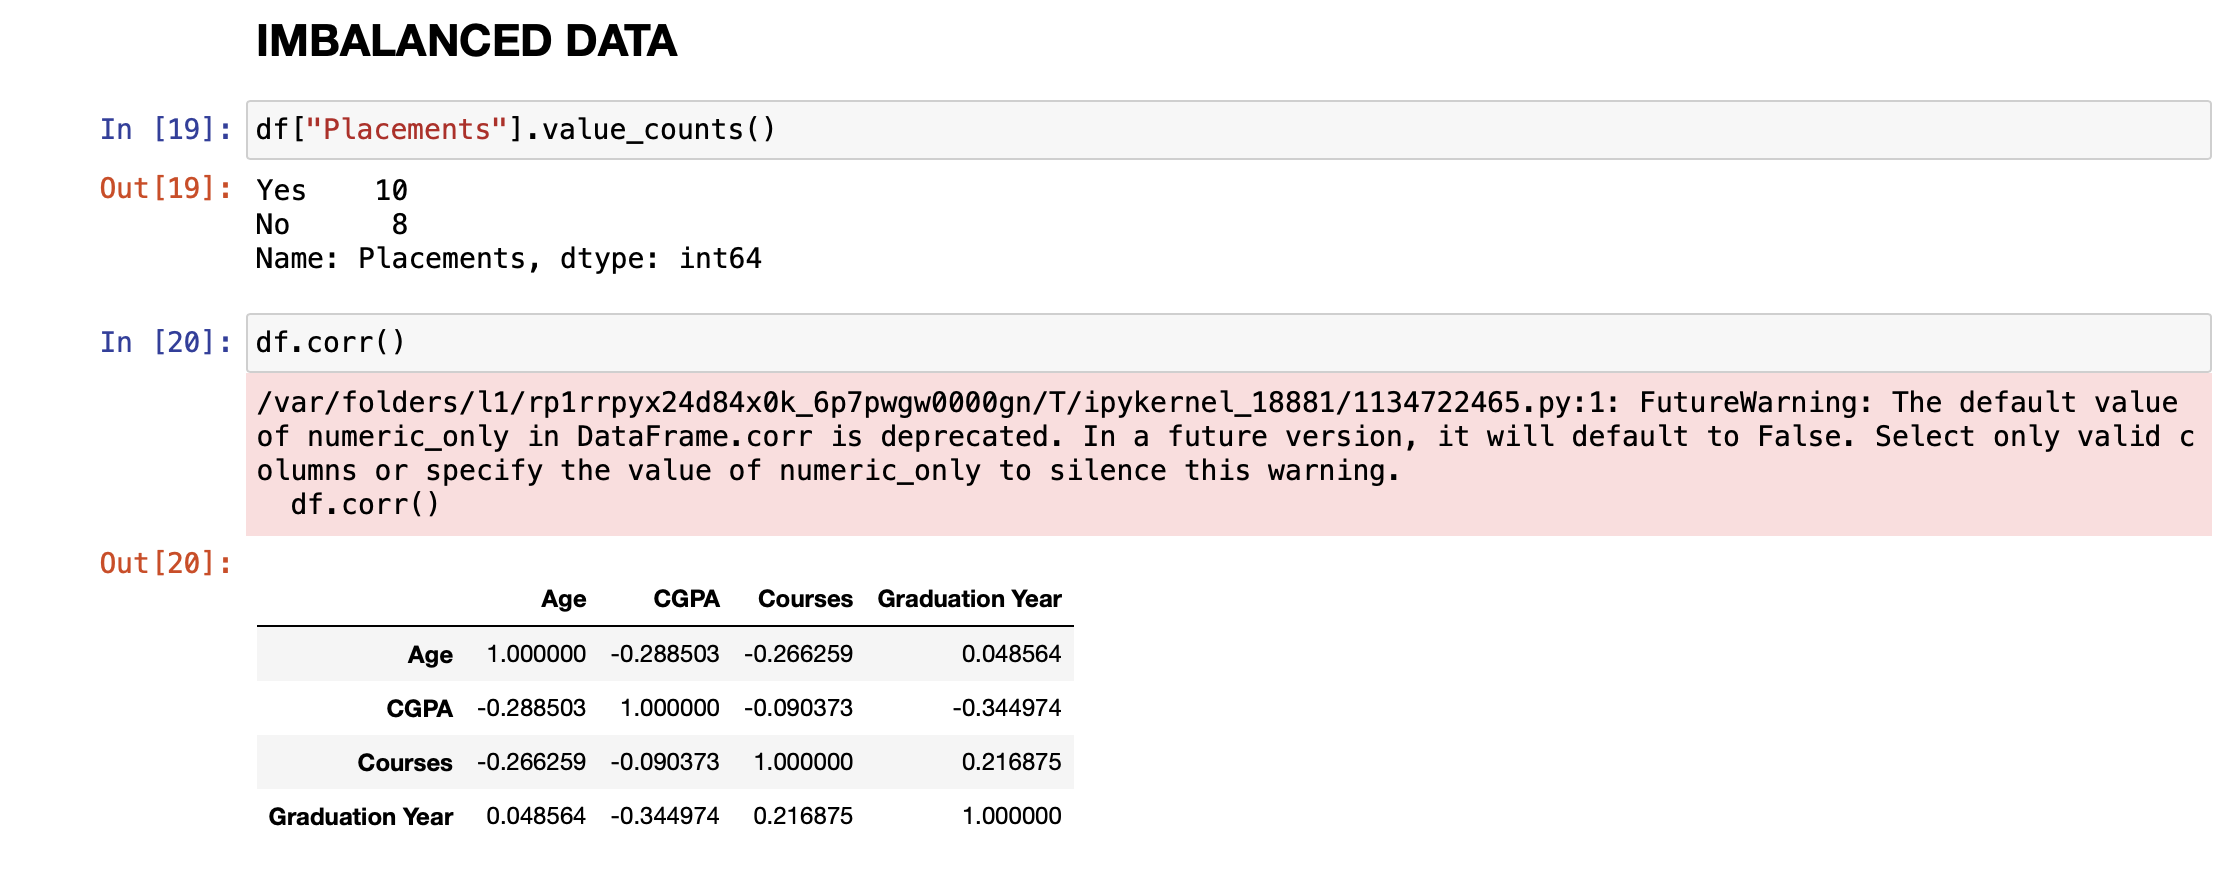
\includegraphics[scale=0.4]{images/8.png}

\section{Undersampling}
\begin{lstlisting}[language=Python]
	from imblearn.under_sampling import RandomUnderSampler
	rus = RandomUnderSampler(random_state=42)
	
	X_res, y_res = rus.fit_resample(X, y)
	X_res_train, X_res_test, y_res_train, y_res_test = train_test_split(X_res,y_res,random_state=1)
	
	
	y_res.value_counts()
\end{lstlisting}
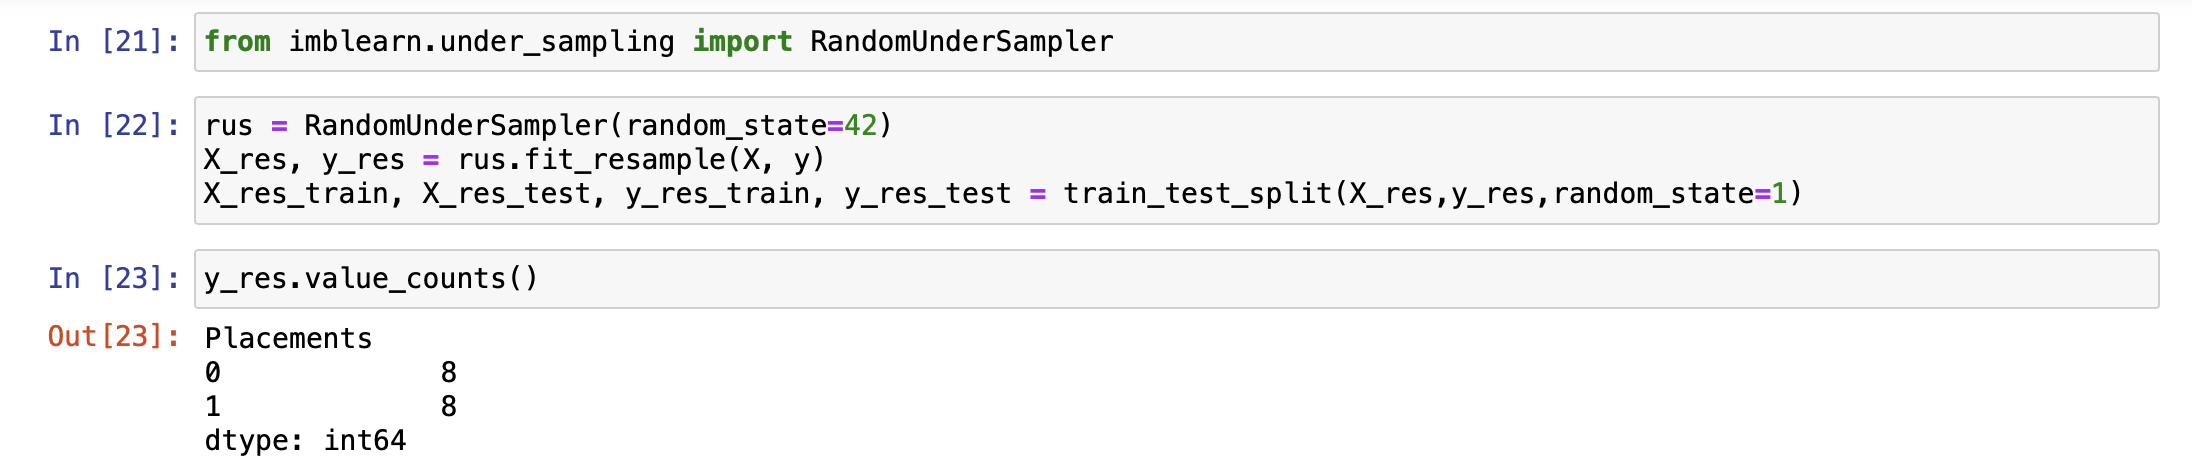
\includegraphics[scale=0.4]{images/9.png}
\section{Undersampling Without PCA}
\begin{lstlisting}[language=Python]
		model1.fit(X_res_train,y_res_train)
		y_pred = model1.predict(X_res_test)
		print(accuracy_score(y_pred,y_res_test))
		print(classification_report(y_pred,y_res_test))
\end{lstlisting}
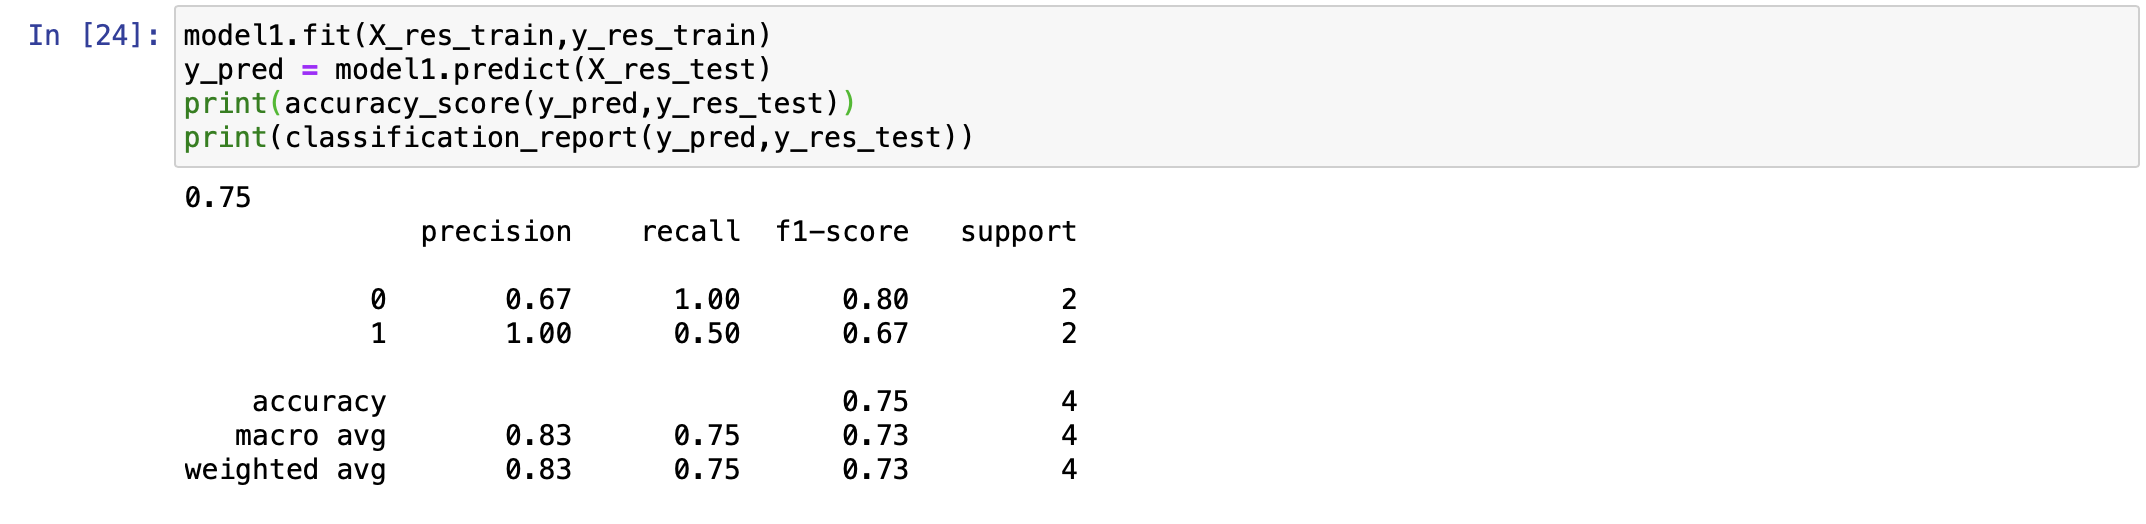
\includegraphics[scale=0.45]{images/10.png}
\section{Undersampling With PCA}
\begin{lstlisting}[language=Python]
	rus1 = RandomUnderSampler(random_state=42)
	X_res, y_res = rus1.fit_resample(X1, y1)
	X_res_train, X_res_test, y_res_train, y_res_test = train_test_split(X_res,y_res,random_state=23)
	
	
	model1.fit(X_res_train,y_res_train)
	y_pred = model1.predict(X_res_test)
	print(accuracy_score(y_pred,y_res_test))
	print(classification_report(y_pred,y_res_test))
	
\end{lstlisting}

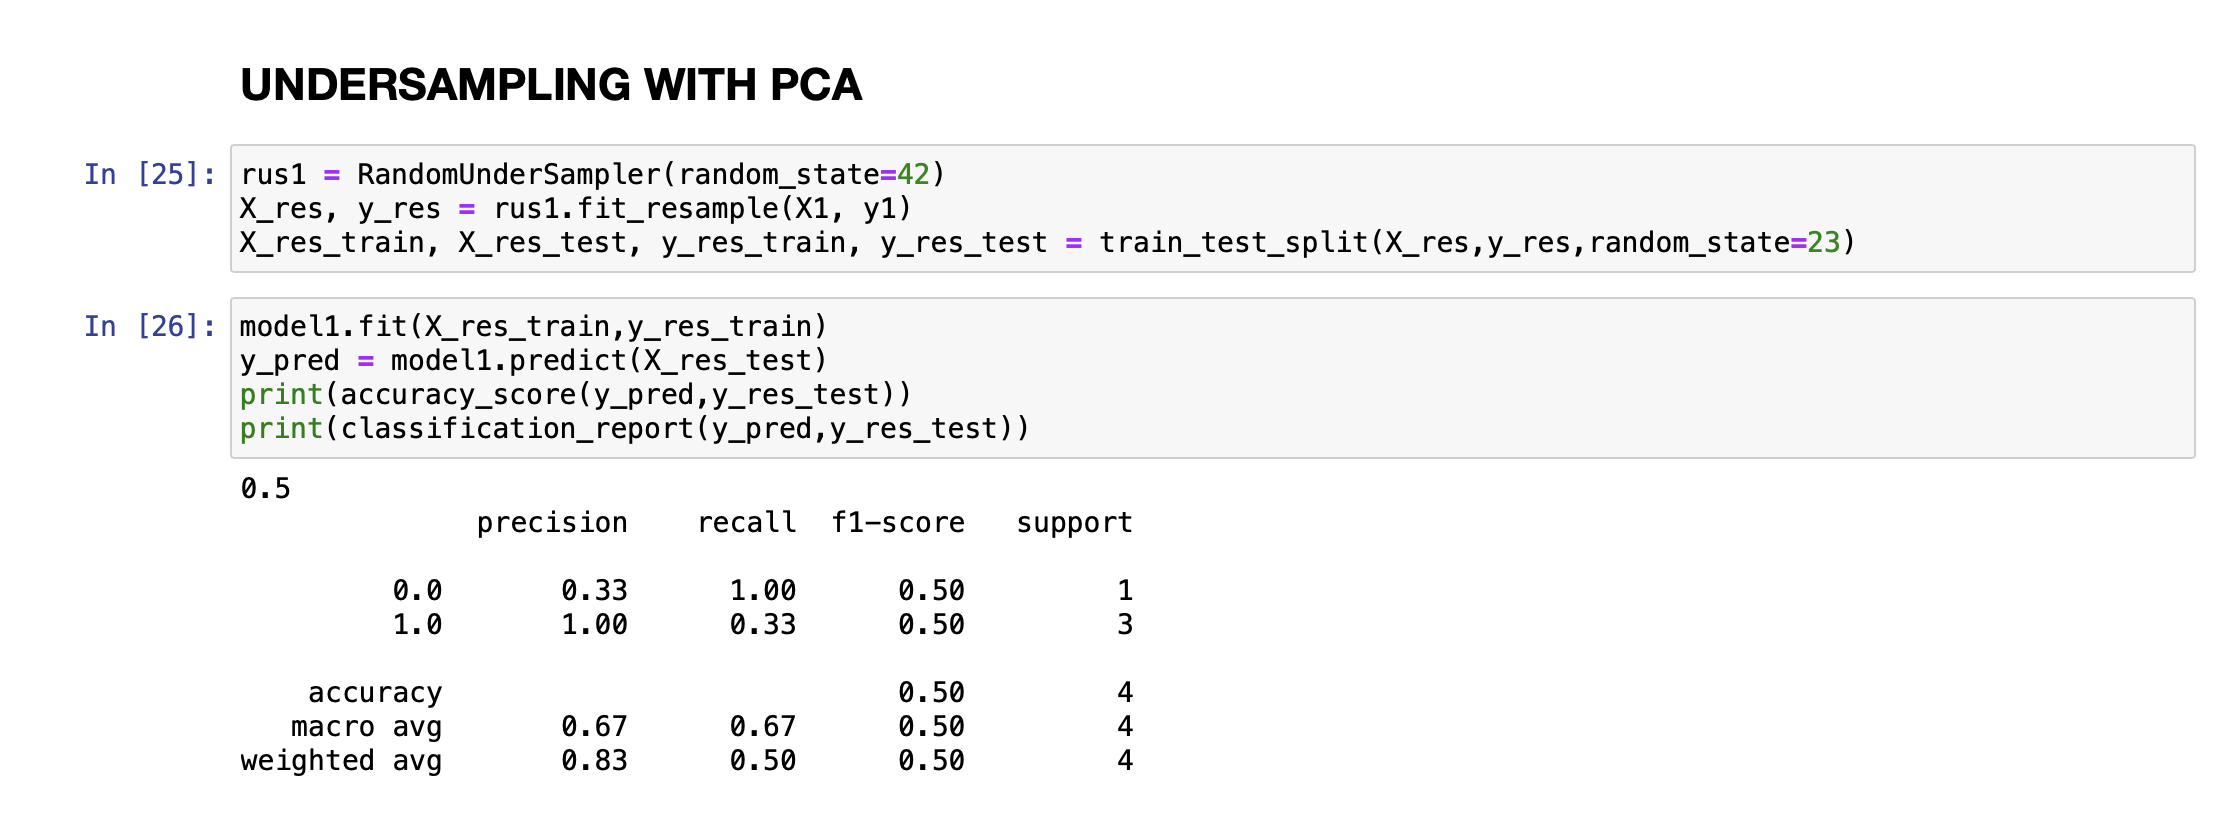
\includegraphics[scale=0.45]{images/11.png}
\section{Oversampling}
\begin{lstlisting}[language=Python]
	from imblearn.over_sampling import RandomOverSampler
	ros = RandomOverSampler(random_state=42)
	X_res, y_res = ros.fit_resample(X, y)
	X_res_train, X_res_test, y_res_train, y_res_test = train_test_split(X_res,y_res,random_state=1)
	
	y_res.value_counts()
	
\end{lstlisting}
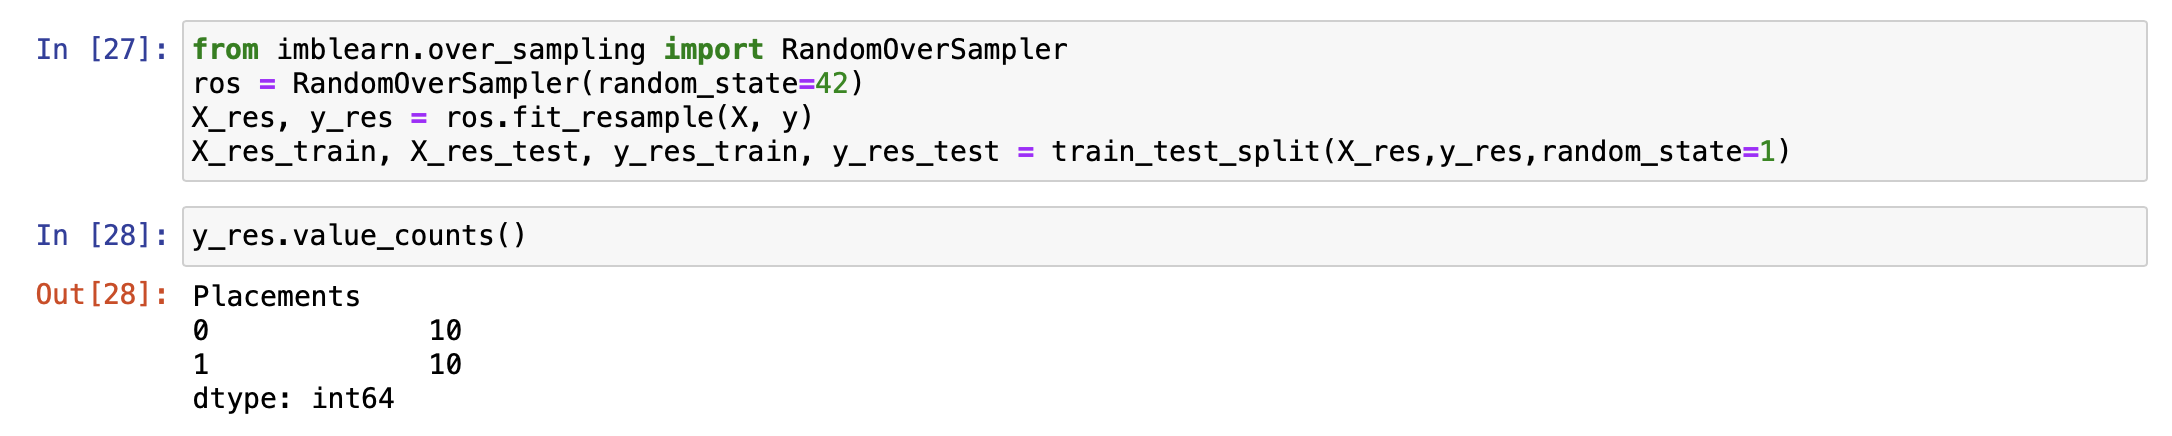
\includegraphics[scale=0.45]{images/12.png}


\section{Oversampling Without PCA}
\begin{lstlisting}[language=Python]
	model1.fit(X_res_train,y_res_train)
	y_pred = model1.predict(X_res_test)
	print(accuracy_score(y_pred,y_res_test))
	print(classification_report(y_pred,y_res_test))
\end{lstlisting}
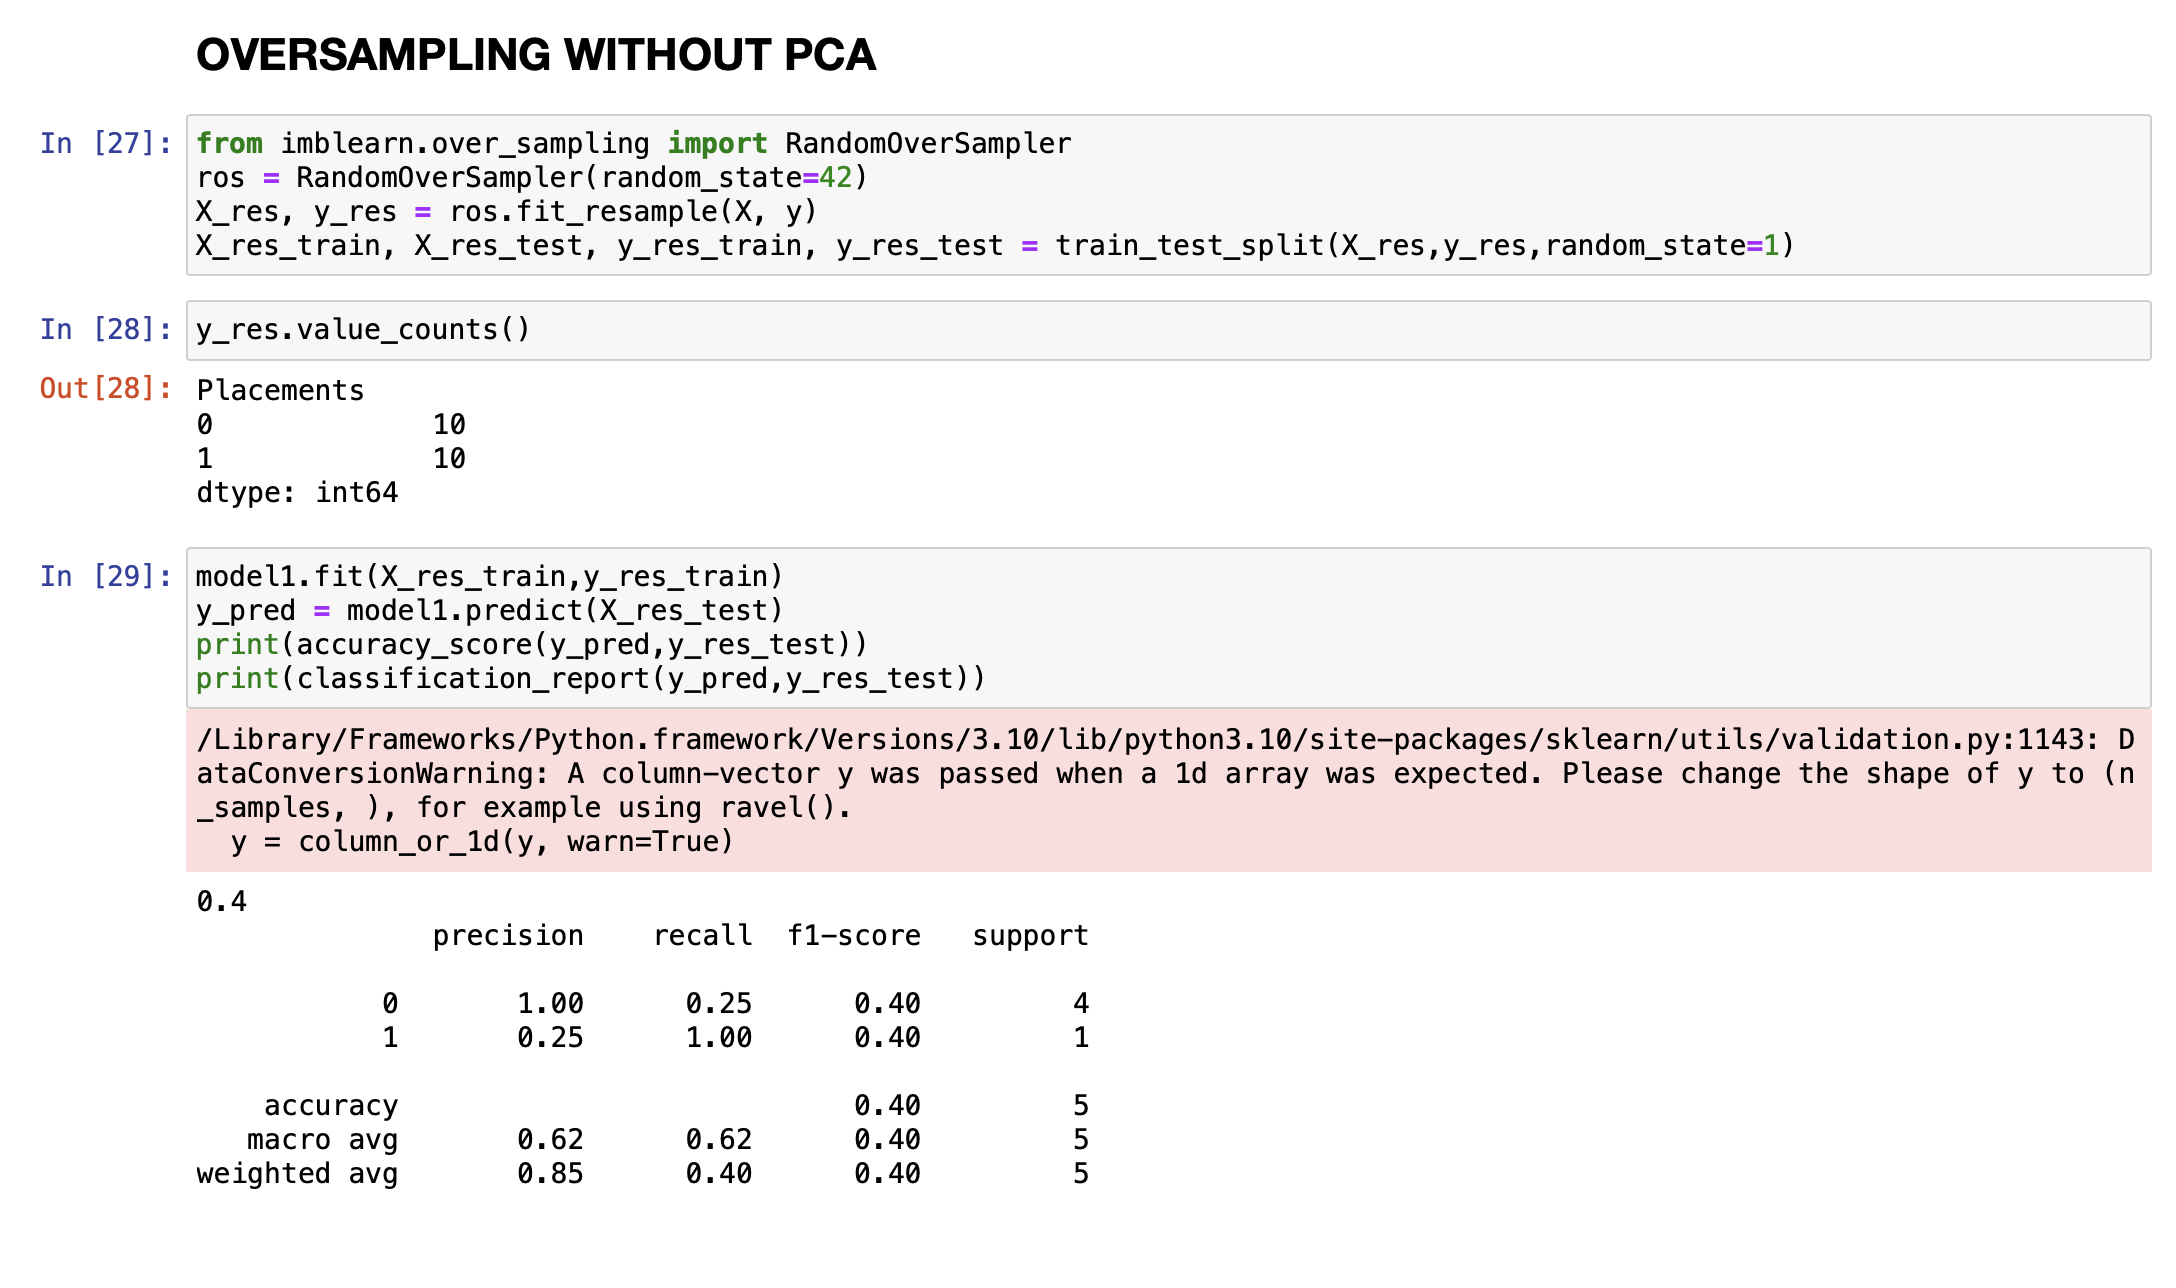
\includegraphics[scale=0.45]{images/13.png}


\section{Oversampling With PCA}
\begin{lstlisting}[language=Python]
	X_res, y_res = ros.fit_resample(X1, y1)
	X_res_train, X_res_test, y_res_train, y_res_test = train_test_split(X_res,y_res,random_state=1)
	
	model1.fit(X_res_train,y_res_train)
	y_pred = model1.predict(X_res_test)
	print(accuracy_score(y_pred,y_res_test))
	print(classification_report(y_pred,y_res_test))
	
\end{lstlisting}
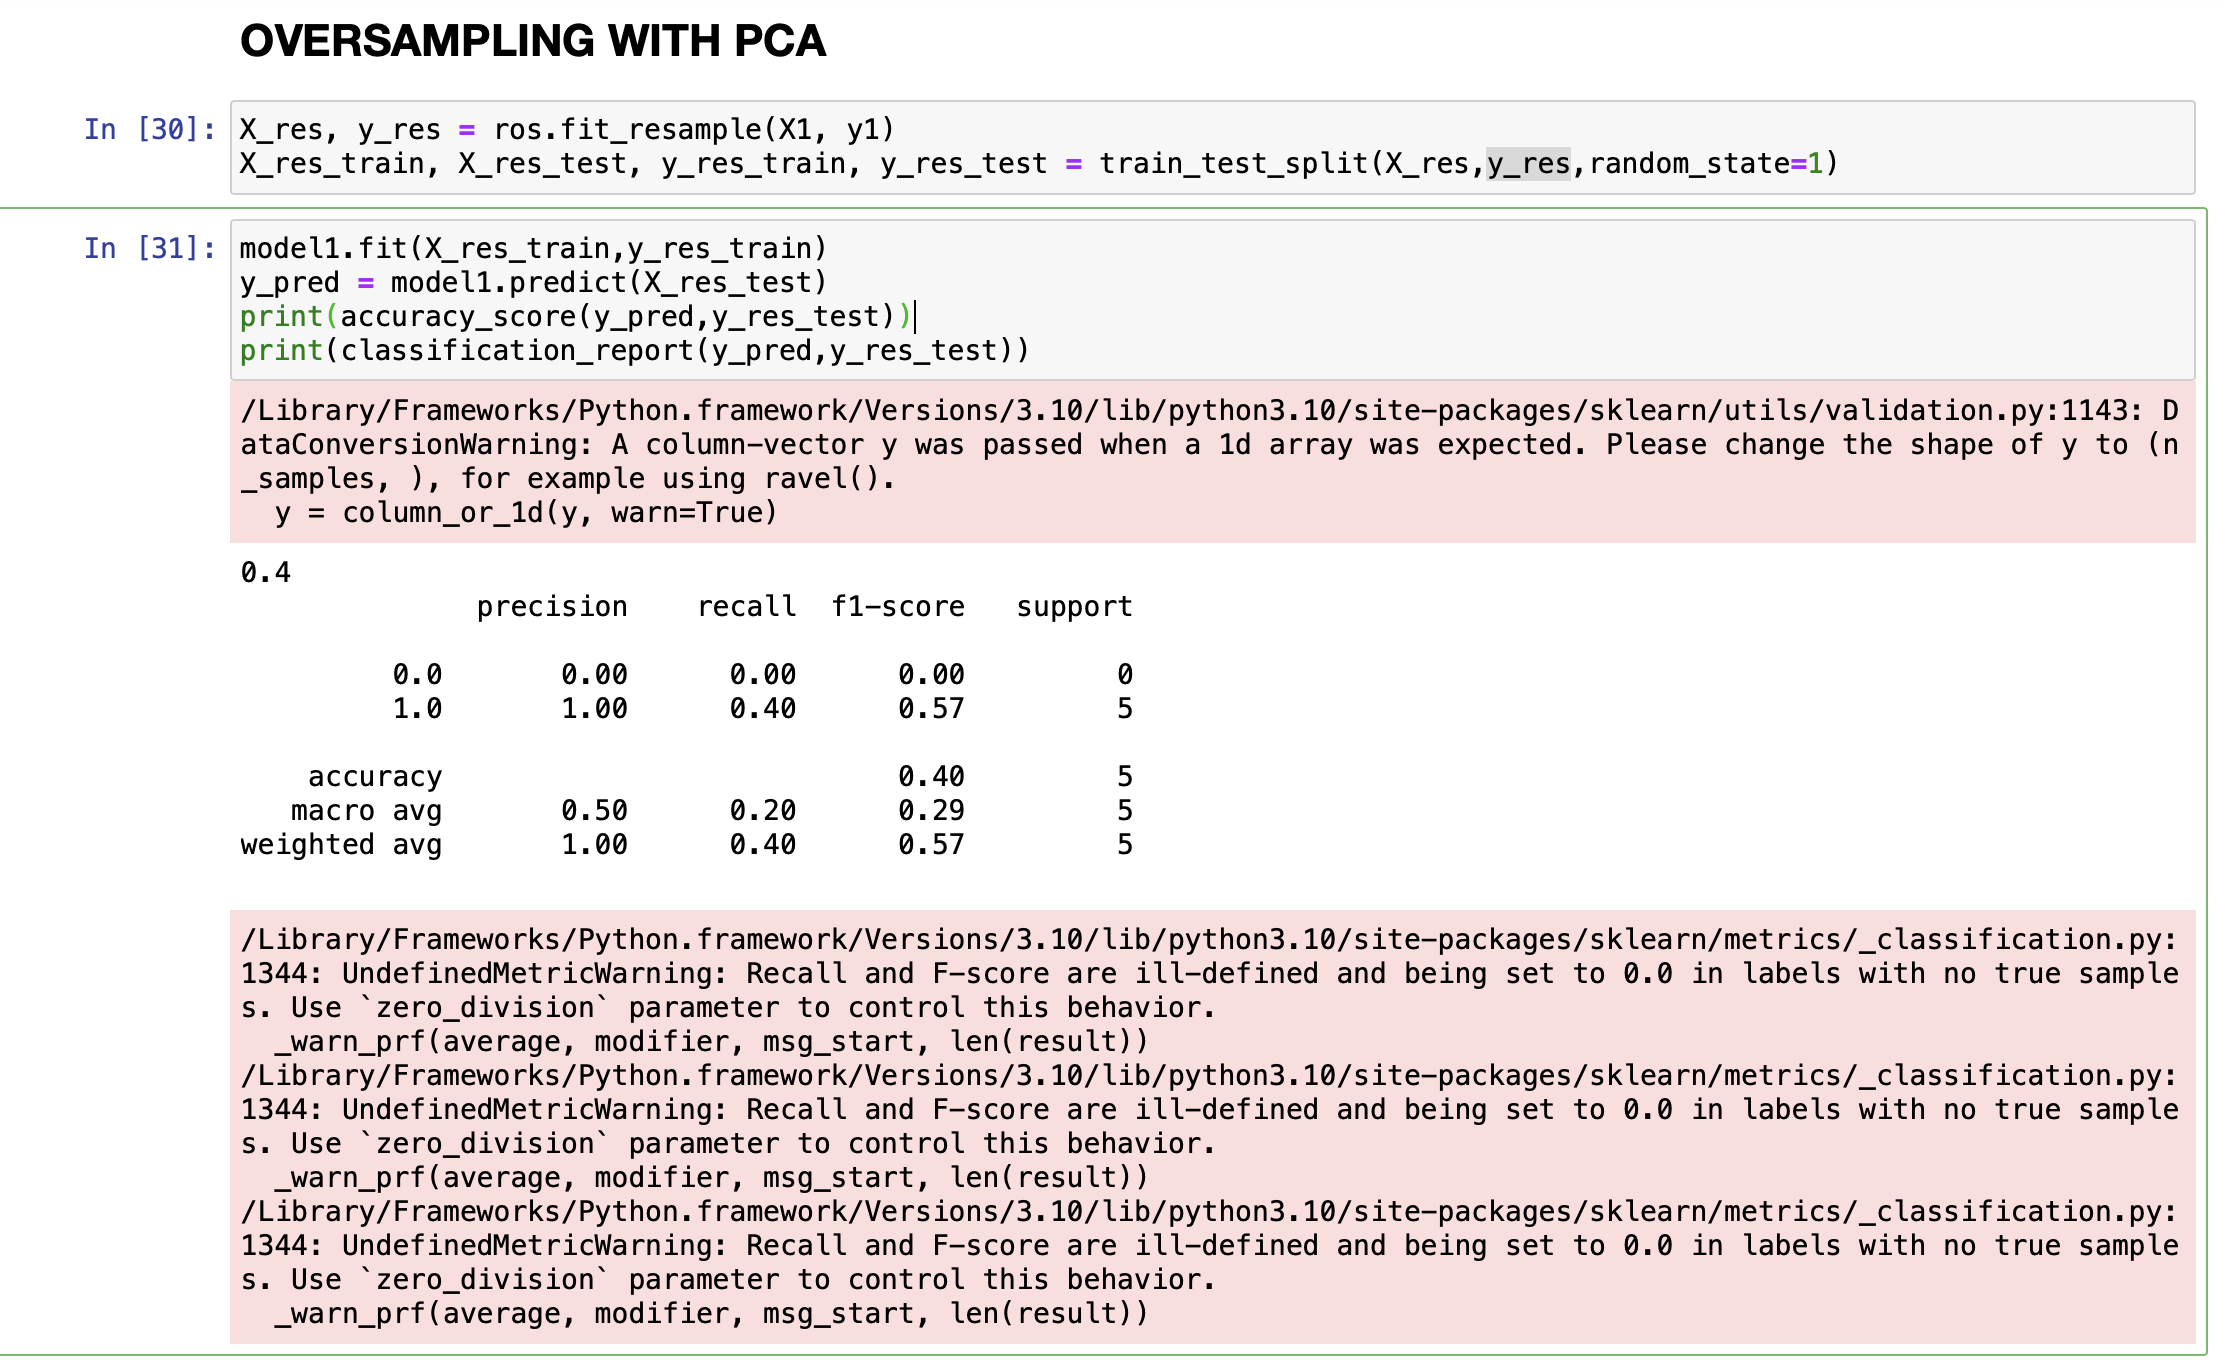
\includegraphics[scale=0.45]{images/14.png}
\end{document}